\chapter{Background}

\section{The MIO and the GHC Runtime}
Haskell programs use a green threading model for concurrency. The GHC runtime system (RTS) is
responsible for the scheduling of these lightweight Haskell threads. Both a single-core “unthreaded”
version and a multicore version \cite{multicoreSupport} of the RTS are available. We will focus on only the multicore
version of the RTS for the remainder of this paper.

In the RTS, a Capability is a virtual CPU for executing Haskell code, the number of which are in the
runtime chosen by the user \cite{multicoreSupport}. Haskell threads are then assigned to these Capabilities to be 
executed. Haskell threads come in three flavors with respect to Capabilities: unbounded, bounded
to a Capability, bounded to an operating system thread. These threads are created with the functions
\texttt{forkIO}, \texttt{forkOn}, and \texttt{forkOS} respectively. 

The definition of the MIO \texttt{EventManager} and notable related
functions are shown in Figure \ref{fig:EventManager}. 

% TODO: Force this to be closer to the text?
\begin{figure}[ht]
  \centering
  \lstinputlisting[language=Haskell]{figures/code/EventManager.hs}
  \caption[\texttt{EventManager} definition and related functions]{
  Definition for \texttt{EventManager} and related functions} 
  \label{fig:EventManager}
\end{figure}


In the definition, \texttt{emBackend} holds an existentially quantified Backend value, allowing for abstraction over
different \texttt{EventManager} Backend implementations, such as \texttt{epoll}-based or \texttt{kqueue}-based. Also of interest is \texttt{emFds},
an array-backed mapping of file descriptors to callbacks, which stores metadata for currently registered requests.

To understand the type signature of the \texttt{registerFd}, specifically how the IO callback is used to wake up a thread,
we need a short detour to explain the Concurrent Haskell \texttt{MVar} synchronization primitive \cite{concurrentHaskell}.
The \texttt{MVar} has the following primitive operations shown in Figure \ref{fig:MVar}. An \texttt{MVar a} can either hold a value of type \texttt{a}, or be empty.

\begin{figure}[H]
  \centering
  \lstinputlisting[language=Haskell]{figures/code/MVar.hs}
  \caption[\texttt{MVar} Functions]{
    \texttt{MVar} Functions
  }
  \label{fig:MVar}
\end{figure}


If \texttt{takeMVar} is called on an empty \texttt{MVar}, the calling Haskell thread will block until another thread calls \texttt{putMVar}
to put a value inside the \texttt{MVar}. Upon successfully taking the \texttt{MVar},
the \texttt{MVar} will become empty.
This Haskell thread blocking is efficient because under the hood,
the \texttt{MVar} is tracked by the RTS, and the thread will sleep until woken up when the RTS realizes the \texttt{MVar} is non-empty.

Thus, the callback passed into \texttt{registerFd} is a \texttt{putMVar} operation is an empty \texttt{MVar}
 Upon calling \texttt{registerFd}, the \texttt{EventManager} will insert a new entry into its emFds
table mapping the file descriptor to the callback. In a separate polling thread,
the \texttt{EventManager} will check for new events, and execute the corresponding appropriate
callbacks from the emFds table. A thread can then call \texttt{takeMVar} to sleep until the \texttt{EventManager}
deems it appropriate to wake up the thread to notify of file descriptor readiness.

In the MIO \texttt{EventManager}, each Capability has an \texttt{EventManager}, and the aforementioned polling
thread is bound to its corresponding Capability.

\clearpage
\section{The \texttt{io\_uring} subsystem}

The \texttt{io\_uring} facility utilizes two circular queues, one for submission and one for completion,
each backed by a shared buffer memory mapping in both user space and kernel space.
Using these two queues, a user process can asynchronously submit and receive results
of system call requests. There is a symmetric relationship between submission versus
reception, and user space versus kernel space. The queues are named from the perspective
of user space. In the submission queue, system call requests, which are written into a
Submission Queue Entry (SQE) struct, are queued into the submission queue by the user process,
and dequeued by the kernel. On the other hand, the results, which are contained in a
Completion Queue Entry (CQE) struct, are queued into the completion queue by the kernel,
and then dequeued by the user process. Submission of an SQE and reading the corresponding
CQE is intended to be equivalent to making the actual system call.

When compared to the polling paradigm, less syscalls are needed.
In the polling paradigm, one syscall is needed to register interest, and
another to perform the actual desired I/O. In the completion paradigm, as
with \texttt{io\_uring}, at most one system call, \texttt{io\_uring\_enter},
is used after queuing the
SQE to let the kernel know of the new entry. It is possible
to batch multiple SQE insertions into one system call, or even require zero
syscalls at all by using a submission queue polling mode that uses a separate
kernel thread to constantly check for new entries.
Completions can then be read from the completion queue without blocking
using atomic instructions. It is also possible to wait on at least a specified
number of completions before returning from the \texttt{io\_uring\_enter} system call.

A key takeaway should be that \texttt{io\_uring} is extremely flexible, and
therefore, has a lot of room to explore optimizations.

The maintainers of \texttt{io\_uring} encourage usage of the \texttt{liburing} bindings
in order to abstract over boilerplate as well as be kernel version agnostic.
Note that in our work however, we use a Haskell library that binds directly to
\texttt{io\_uring} syscalls, similar to liburing itself.

\begin{figure}
  \centering
  \lstinputlisting[language=C]{figures/code/liburing.h}
  \caption[\texttt{liburing io\_uring} wrapper functions]{
  \texttt{liburing} \texttt{io\_uring} wrapper functions}
  \label{fig:liburing.h}
\end{figure}

The core \texttt{liburing} functions used to interface with \texttt{io\_uring} are shown in Figure
\ref{fig:liburing.h}.
To initialize an \texttt{io\_uring} instance, we call
\texttt{io\_uring\_queue\_init}, which after setup,
returns an \texttt{io\_uring} struct containing all relevant state information.
To submit a system call request, we need to first get an available SQE
from the submission queue via \texttt{io\_uring\_get\_sqe}, and fill in the SQE with
our syscall params using a helper function from a family of
\texttt{io\_uring\_prep\_*}
functions. If we want to make an asynchronous read system call,
we use \texttt{io\_uring\_prep\_read}.
If we observe the regular synchronous read system call included
in the same Figure \ref{fig:liburing.h},
we’ll notice similarities to the liburing wrapper version.
Then, to submit all SQEs that we have gotten but not yet submitted, we call
\texttt{io\_uring\_submit}.


In Figure \ref{fig:uring_illustrated}, we have an illustrative diagram of the \texttt{io\_uring} interface and its usage flow.

\begin{figure}[ht]
    \centering
	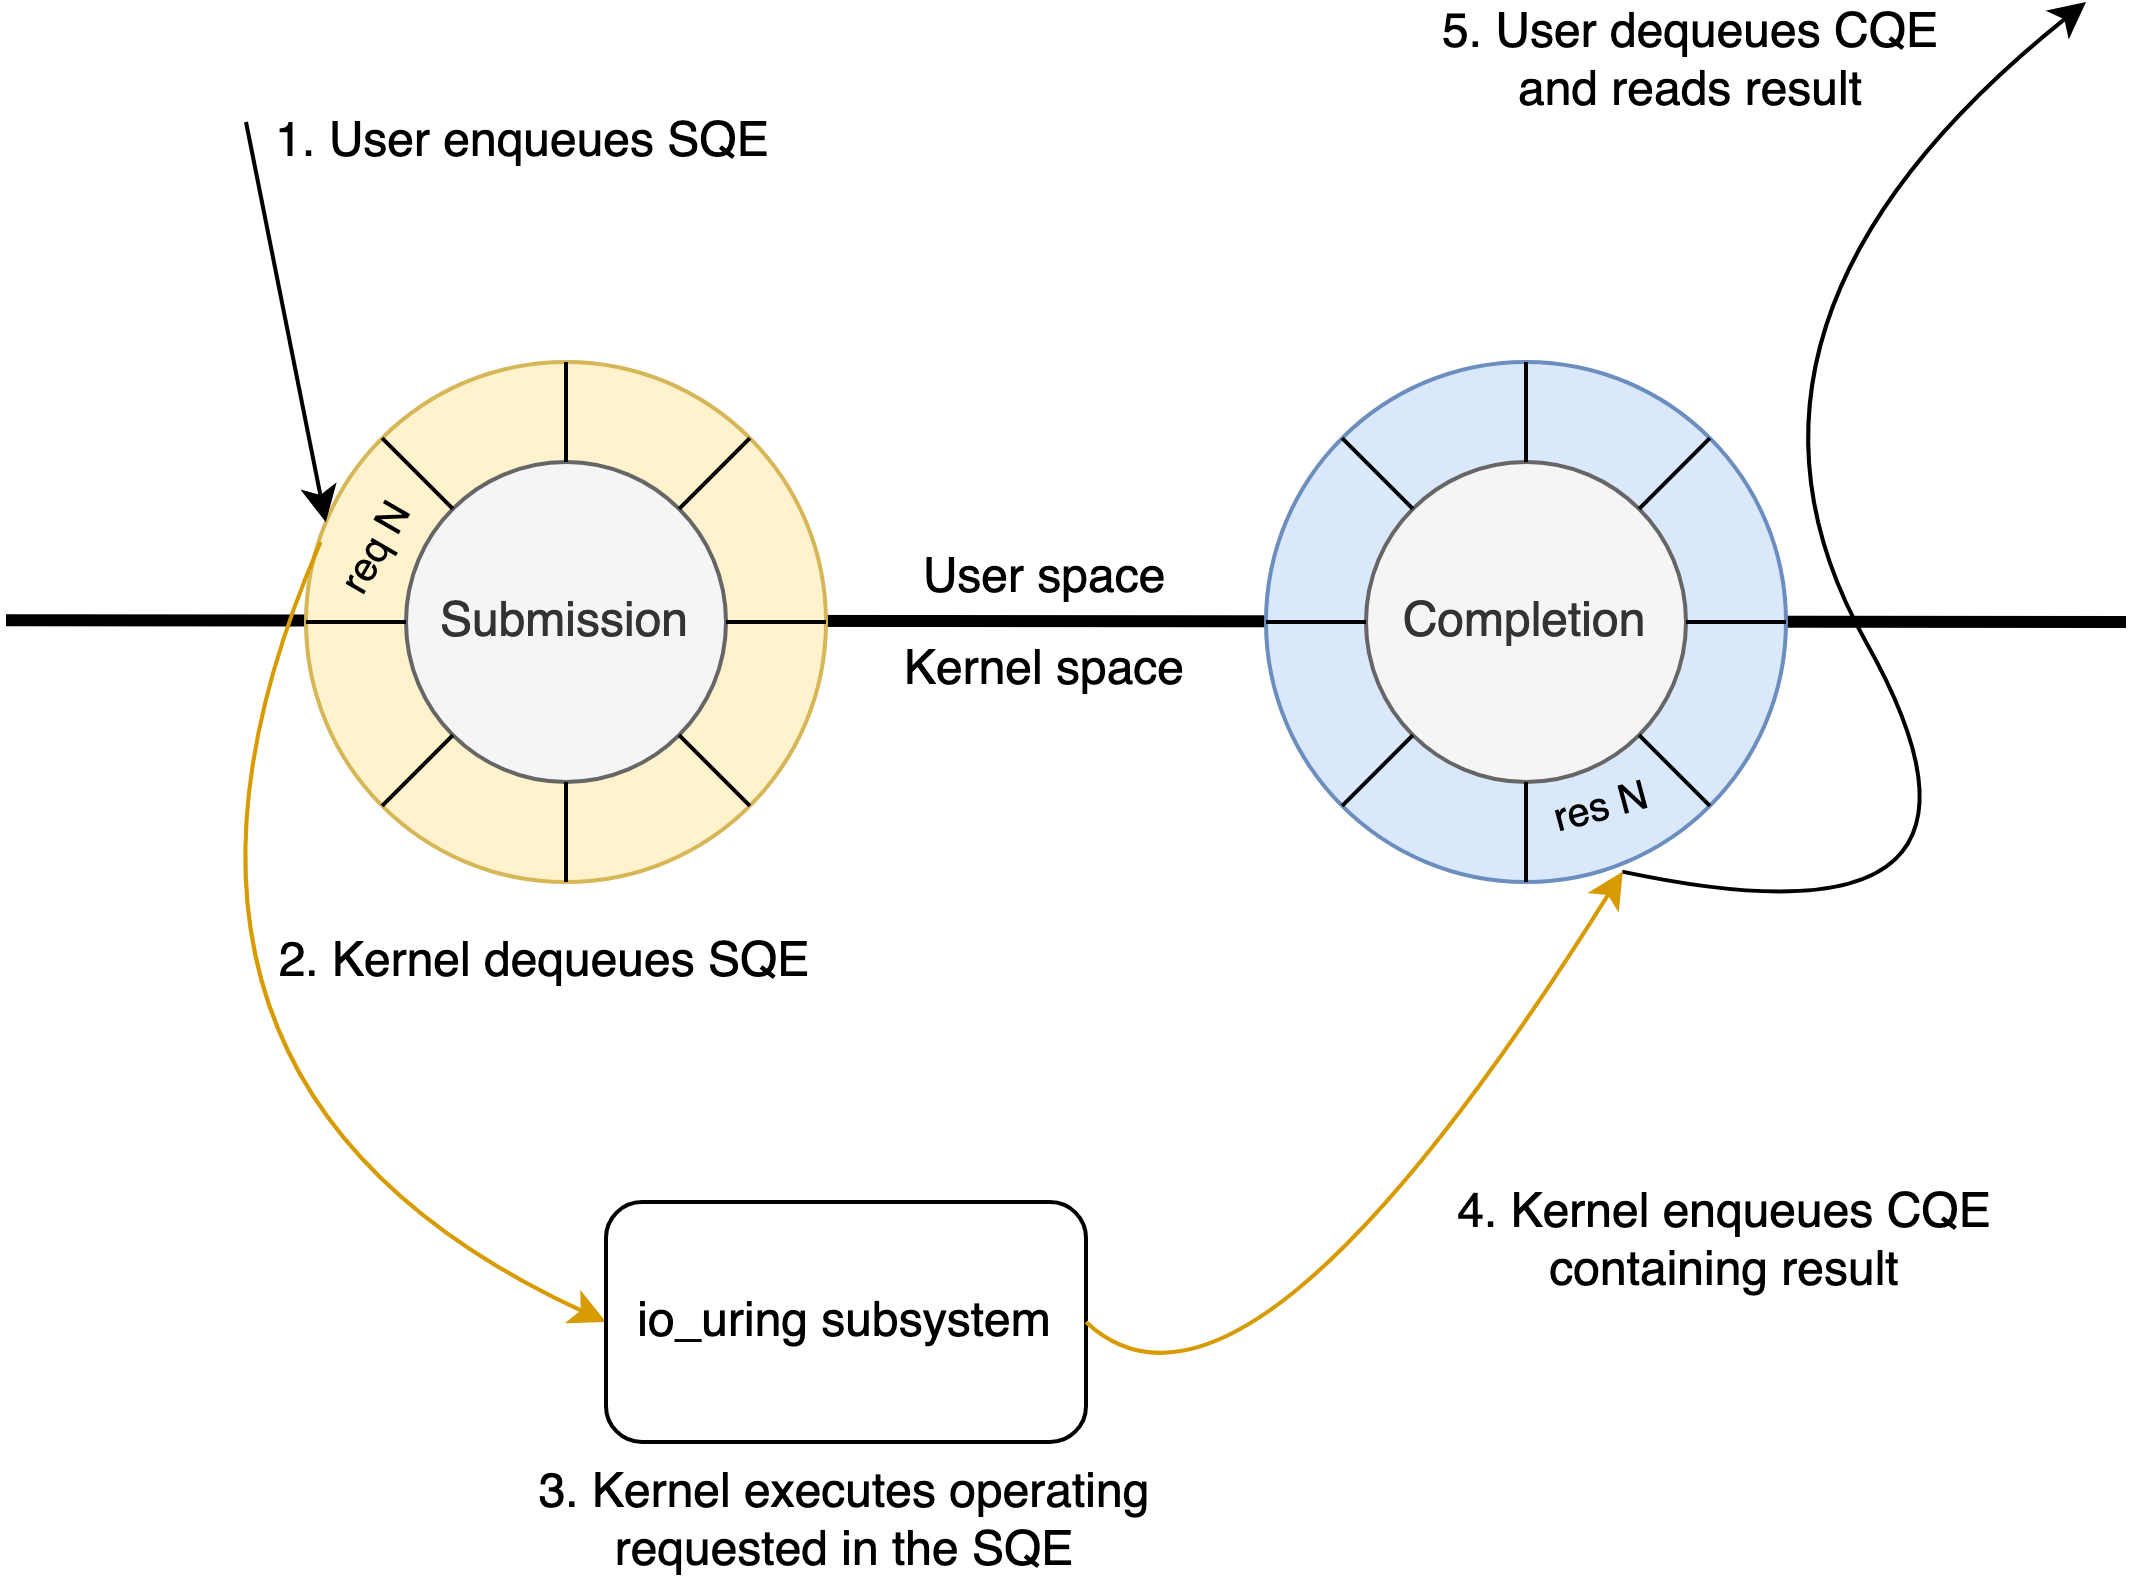
\includegraphics[width=0.85\textwidth]{figures/graphics/uring_illustrated.png}
	\caption[Usage Flow of \texttt{io\_uring}]{
      Usage Flow of \texttt{io\_uring}
	}
	\label{fig:uring_illustrated}
\end{figure} 
